\section{Experimentaci\'on}

Como fue previamente mencionado, la idea ser\'a estudiar qu\'e par\'ametros optimizan el c\'alculo de RTO. Para realizar esto, dividiremos la experimentaci\'on en dos etapas.

Durante la primera etapa, analizaremos c\'omo evoluciona la estimaci\'on de RTO en el cliente con distintas combinaciones de $\alpha$ y $\mathcal{B}$ para un delay fijo y probabilidad de p\'erdida de paquetes nula. A partir de esta experimentaci\'on nos quedaremos con 4 combinaciones de $\alpha$ y $\mathcal{B}$ que a nuestro crtierio son los mejores para estimar el RTO.

Durante la segunda etapa, observaremos c\'omo se comportan las combinaciones anteriores. Para ello volveremos a analizar como evoluciona la estimaci\'on de RTO en el cliente pero, esta vez, iremos variando el delay y la probabilidad de p\'erdida de paquetes. 

\subsection{Etapa Inicial: Estimacion de $\alpha$ y $\beta$}
Con una probabilidad de error nula y un delay de 0.25 segundos, fijaremos los parametros \'optimos de la estimacion del RTO.
Explicar heatmap de los graficos (colores de las barras varian segun magnitud Z del grafico)

\subsubsection{Efectividad en la aproximacion del RTO y el Rtt Real}
	explicar normalizacion de valores y 1-valor
	...graficos 3d de las barras con los alfa y beta variados

\begin{figure}[H]
  \centering	
	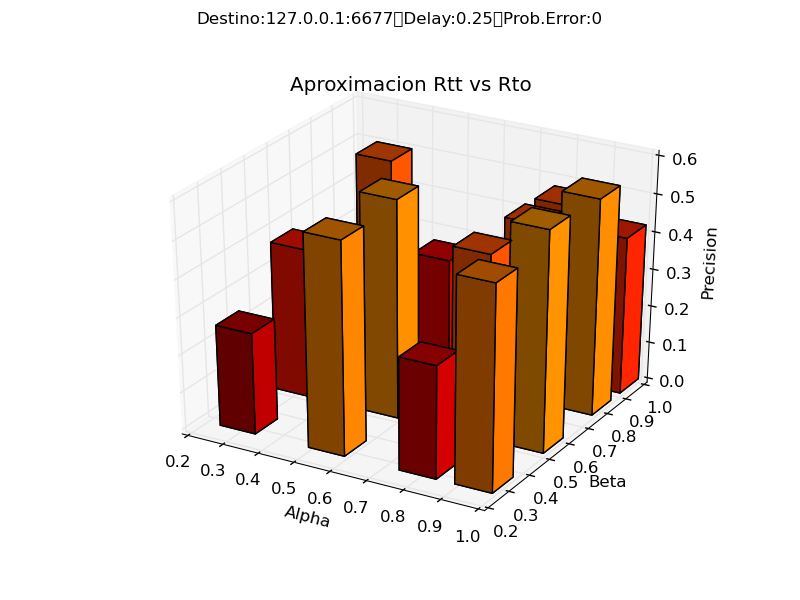
\includegraphics[scale=0.5]{../analisis/graficos_tablas/graficos_en_funcion_de_alfa_y_beta/graficos/rtt_vs_rto.png}
  \caption{Efectividad en la aproximaci\'on del RTO y el RTT Real en funci\'on de $\alpha$ y $\beta$}
	\label{fig:histo-src-sitiotrabajo}
\end{figure}

\subsubsection{Cantidad de retransmisiones}
	...graficos 3d de las barras con los alfa y beta variados

\begin{figure}[H]
  \centering	
	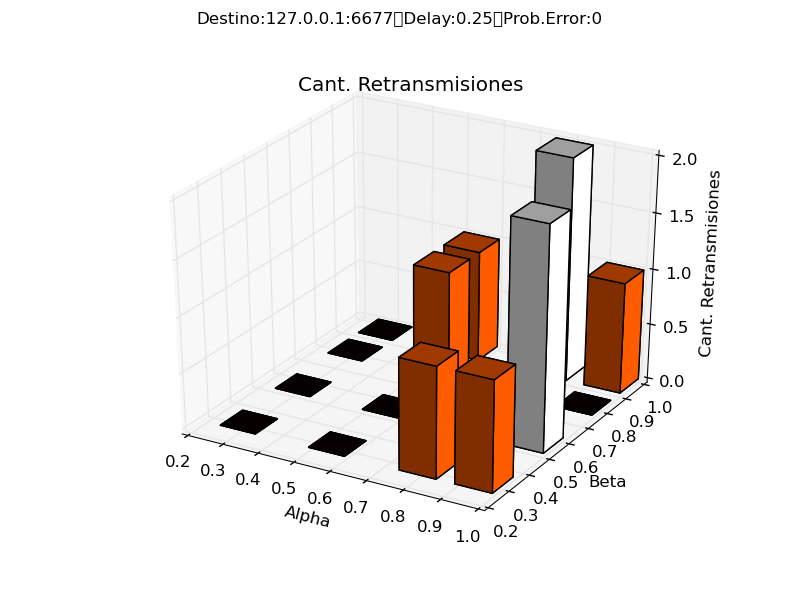
\includegraphics[scale=0.5]{../analisis/graficos_tablas/graficos_en_funcion_de_alfa_y_beta/graficos/retransmisiones.png}
  \caption{Retransmisiones en funci\'on de $\alpha$ y $\beta$}
	\label{fig:histo-src-sitiotrabajo}
\end{figure}

\subsubsection{RTO Estimado}
	...graficos 3d de las barras con los alfa y beta variados

\begin{figure}[H]
  \centering	
	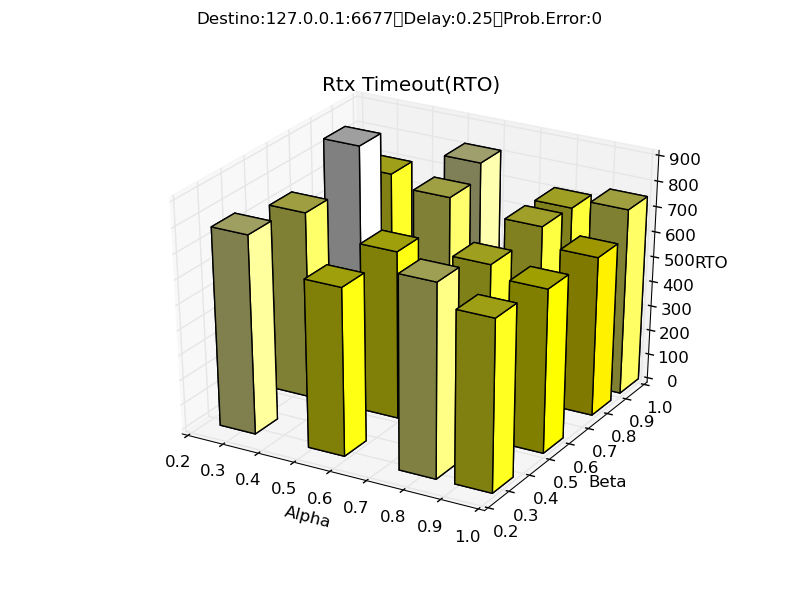
\includegraphics[scale=0.5]{../analisis/graficos_tablas/graficos_en_funcion_de_alfa_y_beta/graficos/rto.png}
  \caption{RTO en funci\'on de $\alpha$ y $\beta$}
	\label{fig:histo-src-sitiotrabajo}
\end{figure}

\subsection{Segunda Etapa - Simulacion de problemas de red: Delay y Errores inducidos con probabilidad}